\documentclass{article}
\usepackage[margin=2cm]{geometry}
\usepackage{natbib}
\usepackage{hyperref}
\usepackage{enumitem}
\usepackage{tikz}
\usetikzlibrary{arrows.meta}
\usetikzlibrary{positioning}

\setlist{nosep} % to reduce space in lists

\setlength{\parskip}{0.5em}
\setlength{\parindent}{0in}

%%%%% NEW MATH DEFINITIONS %%%%%
\usepackage{amsmath,bbm,bm}
\usepackage{amssymb}
\usepackage{amsfonts}
\usepackage{amsthm}
\usepackage{mathtools}

% commands
% global count (no section number)
\newtheorem{thm}{Theorem}%[section]
\newtheorem{lem}{Lemma}
\newtheorem{prop}{Proposition}
\newtheorem{cor}{Corollary}
\newtheorem{conj}{Conjecture}
\newtheorem{aspt}{Assumption}
\newtheorem{claim}{Claim}
\newtheorem{rmk}{Remark}
\newtheorem{commt}{Comment}
\newtheorem{defn}{Definition}

% algorithm
%\usepackage{algorithm, algorithmic}
%\usepackage{algorithm2e}
\usepackage{tabularx}
%\usepackage[table,xcdraw]{xcolor}

% Comments
% \usepackage{xcolor} % already loaded
\newcount\comments  % 0 suppresses notes to selves in text
\comments=1  % TODO: change to 0 for final version
\newcommand{\genComment}[2]{\ifnum\comments=1{\textcolor{#1}{\textsf{\footnotesize #2}}}\fi}
\newcommand{\ed}[1]{\genComment{red}{[EI:#1]}}
\newcommand{\giles}[1]{\genComment{green}{[GH:#1]}}
\newcommand{\kevin}[1]{\genComment{blue}{[KT:#1]}}


% Mark sections of captions for referring to divisions of figures
\newcommand{\figleft}{{\em (Left)}}
\newcommand{\figcenter}{{\em (Center)}}
\newcommand{\figright}{{\em (Right)}}
\newcommand{\figtop}{{\em (Top)}}
\newcommand{\figbottom}{{\em (Bottom)}}
\newcommand{\captiona}{{\em (a)}}
\newcommand{\captionb}{{\em (b)}}
\newcommand{\captionc}{{\em (c)}}
\newcommand{\captiond}{{\em (d)}}


\newcommand\seq[2]{{#1}\!:\!{#2}}
\newcommand\R{\mathbb{R}}
\newcommand\Var{\mathrm{Var}}
\newcommand\var{\Var}
\newcommand\Cov{\mathrm{Cov}}
\newcommand\cov{\Cov}
\newcommand\iid{\mathrm{iid}}
\newcommand\dist{d}
\newcommand\lik{\mathcal{L}}
\newcommand\prob{\mathbb{P}}
\newcommand\E{\mathbb{E}}
\newcommand\loglik{\ell}
\newcommand\process{\texttt{process}}
\newcommand\dimtheta{\mathrm{dim}_{\Theta}}
\newcommand\param{\,;}
\newcommand\giventh\param
\newcommand\given{{\,\vert\,}}
\newcommand\code[1]{\texttt{#1}}
\newcommand\ceil[1]{\lceil #1 \rceil}
\newcommand\floor[1]{\lfloor #1 \rfloor}
\newcommand\1{\bm{1}}


% Highlight a newly defined term
\newcommand{\newterm}[1]{{\bf #1}}


% Figure reference, lower-case.
\def\figref#1{figure~\ref{#1}}
% Figure reference, capital. For start of sentence
\def\Figref#1{Figure~\ref{#1}}
\def\twofigref#1#2{figures \ref{#1} and \ref{#2}}
\def\quadfigref#1#2#3#4{figures \ref{#1}, \ref{#2}, \ref{#3} and \ref{#4}}
% Section reference, lower-case.
\def\secref#1{section~\ref{#1}}
% Section reference, capital.
\def\Secref#1{Section~\ref{#1}}
% Reference to two sections.
\def\twosecrefs#1#2{sections \ref{#1} and \ref{#2}}
% Reference to three sections.
\def\secrefs#1#2#3{sections \ref{#1}, \ref{#2} and \ref{#3}}
% Reference to an equation, lower-case.
\def\eqref#1{equation~\ref{#1}}
% Reference to an equation, upper case
\def\Eqref#1{Equation~\ref{#1}}
% A raw reference to an equation---avoid using if possible
\def\plaineqref#1{\ref{#1}}
% Reference to a chapter, lower-case.
\def\chapref#1{chapter~\ref{#1}}
% Reference to an equation, upper case.
\def\Chapref#1{Chapter~\ref{#1}}
% Reference to a range of chapters
\def\rangechapref#1#2{chapters\ref{#1}--\ref{#2}}
% % Reference to an algorithm, lower-case.
% \def\algref#1{algorithm~\ref{#1}}
% % Reference to an algorithm, upper case.
% \def\Algref#1{Algorithm~\ref{#1}}
% \def\twoalgref#1#2{algorithms \ref{#1} and \ref{#2}}
% \def\Twoalgref#1#2{Algorithms \ref{#1} and \ref{#2}}
% Reference to a part, lower case
\def\partref#1{part~\ref{#1}}
% Reference to a part, upper case
\def\Partref#1{Part~\ref{#1}}
\def\twopartref#1#2{parts \ref{#1} and \ref{#2}}

\def\eps{{\epsilon}}

\def\gN{{\mathcal{N}}}
\def\gX{{\mathcal{X}}}
\def\gY{{\mathcal{Y}}}


\makeatletter
\newcommand*{\addFileDependency}[1]{% argument=file name and extension
\typeout{(#1)}% latexmk will find this if $recorder=0
% however, in that case, it will ignore #1 if it is a .aux or 
% .pdf file etc and it exists! If it doesn't exist, it will appear 
% in the list of dependents regardless)
%
% Write the following if you want it to appear in \listfiles 
% --- although not really necessary and latexmk doesn't use this
%
\@addtofilelist{#1}
%
% latexmk will find this message if #1 doesn't exist (yet)
\IfFileExists{#1}{}{\typeout{No file #1.}}
}\makeatother

\newcommand*{\myexternaldocument}[1]{%
\externaldocument{#1}%
\addFileDependency{#1.tex}%
\addFileDependency{#1.aux}%
}

\newcommand{\off}{\operatorname{off}}
\newcommand{\on}{\operatorname{on}}

\title{Accelerated Inference for Partially Observed Stochastic Processes via Automatic Differentiation}
\author{Kevin Tan}
\date{}

\comments=1

\begin{document}

\maketitle

\begin{center}
    Under the supervision of Giles J. Hooker and Edward L. Ionides
\end{center}


\section{Background}
A partially-observed Markov process (POMP) is defined as follows. Consider an unobserved Markov process $\{X_t, t \geq t_0\}$, and observations $Y_1,...,Y_N$ at timesteps $t_1,..., t_N$. The process is parameterized by an unknown parameter $\theta \in \Theta$, where $X \in \gX, Y \in \gY,$ and finally $\gX, \gY, \Theta \subseteq \R^n$. By a similar decomposition to that in \citet{doucet2009tutorial}, we find that the joint density of $X_{0:N}, Y_{1:N}$ can be factored as
$$f_{X_{0: N}, Y_{1: N}}\left(x_{0: N}, y_{1: N} ; \theta\right)=f_{X_0}\left(x_0 ; \theta\right) \prod_{n=1}^N f_{X_n \mid X_{n-1}}\left(x_n \mid x_{n-1} ; \theta\right) f_{Y_n \mid X_n}\left(y_n \mid x_n ; \theta\right).$$

We call $f_{X_n|X_{n-1}}\left(x_{n} \mid x_{n-1}; \theta\right)$ the process model, writing $\texttt{process}\left(x_n, \theta\right)$ for the simulator corresponding to the above process model, $f_{Y_n|X_n}\left(y_n \mid x_n, \theta\right)$ the measurement model, and will write $y_n^*$ for the actual values of the observations that were observed.

The above are all defined on a single probability space $(\Omega, \Sigma, \prob),$ where $\omega \in \Omega$ denotes an element of the sample space that can be thought of as a random seed. For notational simplicity, we omit the dependence of the likelihood and other suitable calculations on $X_0.$


\begin{figure}[H]
\centering
\begin{tikzpicture}[scale=2]

\node[black] (X_0) at (-3,0) {$X_0$};
\node[black] (Xdot0) at (-2,0) {$...$};
\node[black] (X_{t-1}) at (-1,0) {$X_{t-1}$};
\node[black] (X_t) at (0,0) {$X_t$};
\node[black] (X_{t+1}) at (1,0) {$X_{t+1}$};
\node[black] (Xdot{t+1}) at (2,0) {$...$};
\node[black] (X_T) at (3,0) {$X_T$};
\node[black] (Y_0) at (-3,-1) {$Y_0$};
\node[black] (Ydot0) at (-2,-1) {$...$};
\node[black] (Y_{t-1}) at (-1,-1) {$Y_{t-1}$};
\node[black] (Y_t) at (-0,-1) {$Y_t$};
\node[black] (Y_{t+1}) at (1,-1) {$Y_{t+1}$};
\node[black] (Ydot{t+1}) at (2,-1) {$...$};
\node[black] (Y_T) at (3,-1) {$Y_T$};
\path[->, black] (X_0) edge (Xdot0);
\path[->, black] (Xdot0) edge (X_{t-1});
\path[->, black] (X_{t-1}) edge (X_t);
\path[->, black] (X_t) edge (X_{t+1});
\path[->, black] (X_{t+1}) edge (Xdot{t+1});
\path[->, black] (Xdot{t+1}) edge (X_T);
\path[->, black] (X_0) edge (Y_0);
\path[->, black] (X_{t-1}) edge (Y_{t-1});
\path[->, black] (X_t) edge (Y_t);
\path[->, black] (X_{t+1}) edge (Y_{t+1});
\path[->, black] (X_T) edge (Y_T);
\end{tikzpicture}
\caption{Directed acyclic graph (DAG) of a POMP model.}
\end{figure}

We seek to solve the filtering problem, that is, the problem of estimating
$$p(x_n|y_{1:n}),$$
or the posterior distribution of the state given the current and all previous observations. This can be obtained by Bayesian updating, namely that
\begin{enumerate}
    \item Given a belief on the state space $x_{n-1}$, simulate forward according to $p(\hat x_{n}|x_{n-1})$ to obtain a prediction distribution $\hat x_n$ for the state at time $n$, and
    \item Given a prediction $\hat{x}_n$ at time $n$, observe the measurement $y_n^*$ and perform a Bayesian update to the prediction according to $p(y_n^* | \hat x_{n-1})$ to obtain a belief on the state at time $n$, $x_n$. 
\end{enumerate}

The particle filter is simply the Monte Carlo approximation to this procedure, obtained by maintaining a fixed number $J$ of simulations that we call particles. This induces a mixture Dirac measure on the state space, where we call the belief approximation $x_{n,j}^F$ to the filtering distribution $p(x_n|y_{1:n})$, and the prediction approximation $x_{n,j}^P$ to the prediction distribution $p(x_{n}|y_{1:n-1})$. The intractable integrals involved in the Bayesian update are circumvented with sums over the Dirac measures. 

At a high level, a particle filter keeps track of a set of particles $x_{n,j}$, sequentially approximating (1) the distribution of $X_{n}|y_{1:n-1}^*$ with a mixture Dirac measure $\frac{1}{J}\sum_{j=1}^J \tilde{w}_{n,j}\delta_{x_{n,j}^P}$ via simulation from the process model $p(x_n|x_{n-1})$ and (2) the distribution of $X_{n}|y_{1:n}^*$ with another mixture Dirac measure $\frac{1}{J}\sum_{j=1}^J w_{n,j}\delta_{x_{t,j}^P}$ via a reweighting of the particles in proportion to their likelihood. 

The particle filter approximates the Bayes filter through these two sequences of mixture Dirac measures. The Bayes filter is the "optimal" filter that updates the prediction distribution $p(x_{t}^P|y_{1:t-1}^*)$ with the prediction formula from \cite{sbied_lec3}, 
\begin{equation}
    p(x_{n}^P|y_{1:n-1}^*) = \int p(x_{n-1}^F|y_{1:n-1}^*)p(x_t|x_{t-1}) dx_{n-1},
\end{equation}
and the filtering distribution $p(x_t^F|y_{1:t}^*)$ via Bayes' theorem \citep{sbied_lec3},
\begin{equation}
    p(x_n^F|y_{1:n}^*) = \frac{p(y_n^*|x_n)p(x_n|y_{1:n-1}^*)}{\int p(y_n^*|x_n)p(x_n|y_{1:n-1}^*) dx_n}.
\end{equation}

This therefore provides a simple, general, and computationally efficient solution, yielding an approximation to the filtering distribution and log-likelihood. 


\section{Challenges}



Maximum-likelihood estimation for inference in partially observed stochastic processes, also known as, continuous-state continuous-time hidden Markov models (HMMs), partially-observed Markov processes (POMPs), or partially-observed stochastic nonlinear dynamical systems, is a challenging problem that faces several challenges: 
\begin{enumerate}
    \item Intractable likelihood functions, bypassed with the approaches of simulated likelihood and likelihood-free inference. 
    \item The desire for simulation-based inference without access to the transition density of the latent Markov process, with various methods created by \cite{welch2009abc, wood2010sl, doucet2010pmcmc, ionides08, ionides15}. 
    \item Accurate parameter estimation in the presence of significant Monte-Carlo noise in the likelihood estimate.
\end{enumerate}


Many approaches to inference in these scenarios (such as the EM algorithm, the various Kalman filter variants, and MCMC) either struggle with intractable likelihood functions when the models are complex, or assume access to the probability density of next states given the current state. This is a problem in some critical applications, such as disease modeling, where the models are complex enough such that even obtaining the transition density is an intractable problem. However, the particle filter with the bootstrap proposal, a popular method for solving the filtering problem in partially-observed dynamical systems, provides an unbiased estimate of the likelihood (\cite{delmoral2004feynman}) without requiring evaluation of the transition density of the latent Markov process, enabling an arbitrary model simulator to be plugged into the algorithm.

This is the backbone behind the only simulation-based full-information maximum likelihood method available in the literature thus far, the improved iterated filtering (IF2) algorithm of \citet{ionides15}. \citet{ionides15} utilize the bootstrap filter for perform maximum likelihood estimation with an iterated perturbed Bayes map, successfully tackling challenging problems in epidemiology that available Bayesian methodology fails to solve. 

Still, maximum likelihood parameter estimation can be challenging, especially when the Monte Carlo variance of the evaluation is high and the number of parameters is not small. For example, though in practice the algorithm of \citet{ionides15} converges quickly to a neighborhood of the MLE, it often struggles to successfully optimize the last few-units of the log-likelihood, as we see below in Figure \ref{fig:if2fail}.

\begin{figure}[H]
    \centering
    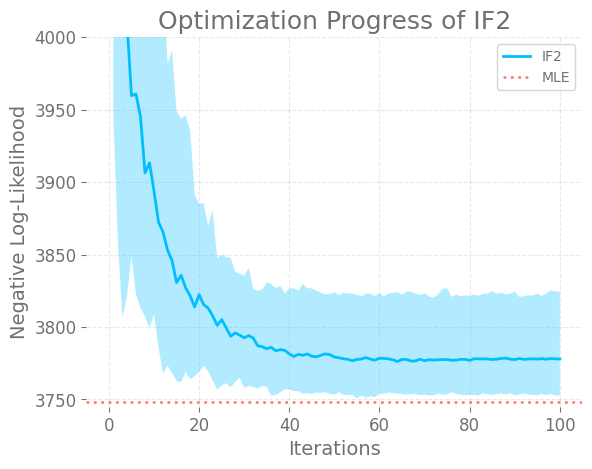
\includegraphics[scale=0.5]{imgs/095/if2fail.png}
    \caption{Failure of iterated filtering on maximum likelihood estimation in the Dhaka cholera model of \cite{king08}. IF2 was run 100 times (with the 0th and 80th quantiles represented with the shaded area), but no run finds the MLE. The best run is about 7.5 log-likelihood units short. }
    \label{fig:if2fail}
\end{figure}

\section{A Potential Solution}

Given the success of stochastic gradient methods in machine learning, it is natural to consider the performance of the procedure of performing gradient descent on the log-likelihood estimate given by the particle filter. We seek to develop a method that performs better than IF2 on this problem, by running IF2 for a few iterations and taking advantage of its quick convergence to a neighborhood of the MLE, and then switching to stochastic gradient descent on the gradient estimate given by running automatic differentiation on the log-likelihood estimate from the particle filter. 



\section{Automatic Differentiation for Particle Filters}

Recent advances in automatic differentiation (AD) for particle filters (\cite{blei2018vsmc, jon2018diffpf, corenflos21, scibior2021dpf, doucet2022particlebased}) have drawn attention to AD as an alternative tool for inference in partially observed stochastic processes with the particle filter. However, these existing approaches either are not yet compatible with the desire for simulation-based inference, or are computationally expensive. 

In particular, only \cite{scibior21}, \cite{blei2018vsmc}, and \cite{corenflos21} have algorithms that are amenable to simulation-based inference without access to transition densities. Though the approach of \citet{corenflos21} is promising, it is computationally expensive, requiring runtime quadratic in the number of particles (unlike other approaches, which run in linear-time). 

\cite{scibior21} show that the estimator of \cite{blei2018vsmc} corresponds to the estimate of the gradient given by differentiating through the vanilla particle filter. This is therefore a very natural estimator for the score. However, \citet{blei2018vsmc} drops high-variance resampling terms from the gradient, leading to bias that does not vanish asymptotically according to \citet{corenflos21}.

A linear-time consistent estimator of the score can be obtained via the estimator of \cite{poyiadjis11}, which \cite{scibior21} show can be obtained through a minor tweak on the particle filter that they call a "stop-gradient trick". However, this estimator has $O(N^2)$ variance, and the stop-gradient trick is not mathematically motivated. 

Of the other methods that are not compatible with simulation-based inference, \citet{doucet2022particlebased} provide another promising fixed-lag smoothing-based approach, but requires either (1) access to the process model transition densities or (2) the special case where the transition density factors into a policy that selects actions (in the reinforcement learning sense) and a deterministic model that maps states and actions to next-timestep states. 

\section{Our Contributions}

Previous research on AD for particle filters has struggled with various issues: 
\begin{enumerate}
    \item Bias, if the discontinuous nature of particle resampling is ignored.
    \item High Monte Carlo variance, if continuity corrections lead to numerical instability.
    \item High computational cost, for algorithms which involve pairwise interactions between particles, marginalization, smoothing or optimal transport.
    \item Reduced applicability for algorithms which lose or fail to take advantage of the simulation-based capabilities of the bootstrap filter.
\end{enumerate}

We develop a new approach to statistical inference via AD for particle filters which addresses these concerns. We develop a new theoretical framework that encompasses existing methods, and addresses the seemingly incompatible paradox of differentiating through a Monte-Carlo algorithm with discontinuous resampling.

This is done through the construction of a smooth extension to the particle filter, as well as a \textbf{Measurement Off-Policy-$\alpha$} (MOP-$\alpha$) family of algorithms that (informally) encompasses the special case of AD of a vanilla PF (recovering the gradient estimator of \citet{blei2018vsmc}) when $\alpha=0$, and the DPF algorithm from \citet{scibior2021dpf} (that recovers the gradient estimator from \citet{poyiadjis11}) when $\alpha=1$. When $\alpha \in (0,1)$, this provides opportunities for optimizing a bias/variance tradeoff. 

We will show that these off-policy particle filters successfully target the posterior, recover desirable gradient estimates previously encountered in the literature, and possess other desirable theoretical properties. This entails novel proofs showing a strong law of large numbers for triangular arrays under bounded particle weights and functionals, with the application of showing that a suitably reweighted particle filter still targets the posterior, even when resampling is carried out under some other arbitrary categorical distribution.


In practice, we propose a hybrid algorithm that we call \textbf{Iterated Filtering with Automatic Differentiation (IFAD)} that warm-starts gradient ascent (or a similar iterative first or second-order gradient method) with a coarse solution obtained from a few rounds of iterated filtering. Promising preliminary numerical results indicate that this can beat current state-of-the-art methods on a challenging scientific benchmark problem.

\bibliography{bib-ifad,bib-ref}
\bibliographystyle{apalike}


\end{document}
